\documentclass[conference]{IEEEtran}
\IEEEoverridecommandlockouts
% The preceding line is only needed to identify funding in the first footnote. If that is unneeded, please comment it out.
\usepackage{cite}
\usepackage{amsmath,amssymb,amsfonts}
\usepackage{algorithmic}
\usepackage{graphicx}
\usepackage{textcomp}
\usepackage{xcolor}
\def\BibTeX{{\rm B\kern-.05em{\sc i\kern-.025em b}\kern-.08em
    T\kern-.1667em\lower.7ex\hbox{E}\kern-.125emX}}
\begin{document}

\title{Textile Industry in Bangladesh\\
{\footnotesize \textsuperscript{*}The Backbone Of the Economy Of Bangladesh}
\thanks{Identify applicable funding agency here. If none, delete this.}
}

\author{\IEEEauthorblockN{1\textsuperscript{st} Ahmed Reza Riday(200101022)}
\IEEEauthorblockA{\textit{Computer Science And Engineering} \\
\textit{Bangladesh Army University Of Science And Technology}\\
Saidpur, Bangladesh \\
ahmedreza98shams@gmail.com}
\and
\IEEEauthorblockN{2\textsuperscript{nd} Md. Showmik Hasan(200101034)}
\IEEEauthorblockA{\textit{Computer Science And Engineering} \\
\textit{Bangladesh Army University Of Science And Technology}\\
Saidpur, Bangladesh \\
cse.200101034@gmail.com}
\and
\IEEEauthorblockN{3\textsuperscript{rd} Huzaifa Hassan(200101003)}
\IEEEauthorblockA{\textit{Computer Science And Engineering} \\
\textit{Bangladesh Army University Of Science And Technology)}\\
Saidpur, Bangladesh \\
cse.200101003@gmail.com}
\and
\IEEEauthorblockN{4\textsuperscript{th} Shafein Sadia Islam(200101045)}
\IEEEauthorblockA{\textit{Computer Science And Engineering} \\
\textit{Bangladesh Army University Of Science And Technology}\\
Saidpur, Bangladesh \\
cse.200101045@gmail.com}
\and
\IEEEauthorblockN{5\textsuperscript{th} Bonnhi Shikha Dutta(200101029)}
\IEEEauthorblockA{\textit{Computer Science And Engineering} \\
\textit{Bangladesh Army University Of Science And Technology}\\
Saidpur, Bangladesh \\
cse.200101029@gmail.com}
\and
\IEEEauthorblockN{6\textsuperscript{th} Md. Mostofa Wadud(200101020)}
\IEEEauthorblockA{\textit{Computer Science And Engineering} \\
\textit{Bangladesh Army University Of Science And Technology}\\
Saidpur, Bangladesh \\
cse.200101020@gmail.com}
}

\maketitle

\begin{abstract}
The textile and clothing industries provide a single source of growth in Bangladesh's rapidly developing economy. Exports of textiles and garments are the principal source of foreign exchange earnings. By 2002 exports of textiles, clothing, and ready-made garments (RMG) accounted for 77\% of Bangladesh's total merchandise exports.

In 1972, the World Bank approximated the gross domestic product (GDP) of Bangladesh at US\$6.29 billion, and it grew to \$368 billion by 2021, with \$46 billion of that generated by exports, 82\% of which was ready-made garments. As of 2016 Bangladesh held the 2nd place in producing garments just after China. Bangladesh is the world's second-largest apparel exporter of western fast fashion brands. Sixty percent of the export contracts of western brands are with European buyers and about thirty percent with American buyers and ten percent to others. Only 5\% of textile factories are owned by foreign investors, with most of the production being controlled by local investors. In the financial year 2016-2017 the RMG industry generated US\$28.14 billion, which was 80.7\% of the total export earnings in exports and 12.36\% of the GDP; the industry was also taking on green manufacturing practices.


\end{abstract}

\begin{IEEEkeywords}
textiles,gdp,rmg(ready-made garments),women empowerment,export
\end{IEEEkeywords}

\section{Introduction}
The textile industries in the Bangladesh is a main sector of country economy. Bangladeshi Textiles industry has a famous reputation in the world’s competitive garments market. The textile industry of Bangladesh is specialized in textile goods, knitwear, and woven apparels. These products are top in grabbing the export income for the country.

\section{Trade agreements}

\subsection{1974 the Multi Fibre Arrangement (MFA) and the Daewoo of South Korea}

Starting in 1974 the Multi Fibre Arrangement (MFA) in the North American market ensured that trade in textiles and garments remained the most regulated in the world. Among other things the MFA set quotas on garments exports from the newly industrialising countries of Asia, but had exceptions, most notably the state of Bangladesh. Entrepreneurs from quota-restricted countries like South Korea began "quota hopping" seeking quota-free countries that could become quota-free manufacturing sites. The export-oriented readymade garment industry emerged at this time. Daewoo of South Korea was an early entrant in Bangladesh, when it established a joint venture on 27 December 1977 with Desh Garments Ltd. making it the first export oriented ready-made garment industry in Bangladesh. After only one year in which 130 Desh supervisors and managers received free training from Daewoo in production and marketing at Daewoo's state-of-the-art ready-made garment plant in Korea, 115 of the 130 left Desh Garments Ltd. and set up separate private garment export firms or began working for other newly formed export-oriented RMG companies with new garment factories in Bangladesh for much higher salaries than Desh Garments Ltd offered.

Global restructuring processes, including two non-market factors, such as quotas under Multi Fibre Arrangement (MFA) (1974–2005) in the North American market and preferential market access to European markets, led to the "emergence of an export-oriented garment industry in Bangladesh in the late 1970s." It was uncertain what the phase out of the MFA meant for the Bangladeshi RMG industry. However, surpassing all doubts, the industry continued to succeed and dominate on a global level.

The garment industry in Bangladesh became the main export sector and a major source of foreign exchange starting in 1980, and exported about US\$5 billion in 2002. In 1980 an export processing zone was officially established in at the port of Chittagong.

By 1981, 300 textile companies, many small ones had been denationalized often returned to their original owners. In 1982, shortly after coming to power following a bloodless coup, President Hussain Muhammad Ershad introduced the New Industrial Policy (NPI), most significant move in the privatization process, which denationalized much of the textile industry, created export processing zones (EPZs) and encouraged direct foreign investment. Under the New Industrial Policy (NPI) 33 jute mills and 27 textile mills were returned to their original owners.

In 1985 the US and Canada actually imposed import quotas of their own, with no international agreement, on Bangladeshi textiles. However, Bangladesh was able to meet demand for every quota each year and was able to successfully negotiate for higher quotas for subsequent years.

The export of ready-made garments (RMG) increased from US\$3.5 million in 1981 to \$10.7 billion in 2007. Apparel exports grew, but initially, the ready-made garments RMG industry was not adequately supported by the growth up and down the domestic supply chain (e.g., spinning, weaving, knitting, fabric processing, and the accessories industries).

From 1995 to 2005 the WTO Agreement on Textiles and Clothing (ATC) was in effect, wherein more industrialized countries consented to export fewer textiles while less industrialized countries enjoyed increased quotas for exporting their textiles. Throughout the 10-year agreement, Bangladesh's economy benefited from quota-free access to European markets and desirable quotas for the American and Canadian markets.

\section{World markets}
As of 2011 Bangladesh was second largest ready-made garments (RMG) manufacturer after China, by the next five years Bangladesh will become the largest ready-made garments manufacturer. Bangladesh was the sixth largest exporter of apparel in the world after China, the EU, Hong Kong, Turkey and India in 2006. In 2006 Bangladesh's share in the world apparel exports was 2.8\%. The US was the largest single market with US\$3.23 billion in exports, a 30\% share in 2007. Today, the US remains the largest market for Bangladesh's woven garments taking US\$2.42 billion, a 47\% share of Bangladesh's total woven exports. The European Union remains the largest regional destination - Bangladesh exported US\$5.36 billion in apparel; 50\% of their total apparel exports. The EU took a 61\% share of Bangladeshi knitwear with US\$3.36 billion exports.
According to a 2011 report by international consulting firm McKinsey \& Company, 80 percent of American and European clothing companies planned to move their outsourcing from China, where wages had risen, and were considering Bangladesh as the "next hot spot" making it the "next China" offering 'the lowest price possible' known as the China Price, the hallmark of China's incredibly cheap, ubiquitous manufacturers, much "dreaded by competitors."\\

\subsection{Abbreviations and Acronyms}\label{AA}
RMG = Ready-Made Garments\\
NPI = New Industrial Policy\\
EPZ = Export Processing Zone \\
WTO = World Trade Organization\\
ATC = Agreement on Textiles and Clothing\\


\subsection{ Environmental scenario}
\begin{itemize}
\item Bangladesh’s textile industry can be divided into three main categories: public sector, handloom sector, and the organized private sector, The private sector is the fastest growing sector in the country. Most of these industrial units are located along the banks of the rivers, which provide transportation for incoming raw materials and outgoing finished products. Unfortunately, as a consequence, industrial units drain effluents directly into the rivers without any consideration of the environment.
\item Textiles are one of the most problematic industries for the water sector. A complex mixture of hazardous chemicals, both organic and inorganic, is discharged into the water bodies from all these industries, usually without treatment. The highest number of industrial locations in the country is in the North Central (NC) region, which comprises just under half of the total sector.
\item About 33 per cent of the industries in the NC region are textiles, finished garments and tanneries, of which Dhaka district accounts for almost half and Narayanganj about 32 per cent. The most polluting industrial units listed in 1986 included 298 textile mills, which rose to 365 units in the recent statistics of DoE. Around 50% of these are small-scale industries and their contributions to environmental pollution are summarized in the Table1 in terms of wastewater (m3) and biological oxygen demand (BOD load, kg/day) discharged into the inland surface water discharged per day.
\item The water samples from point sources, upstream areas and deep tube wells were collected and analyzed for Na, K, Mg, Ca, Fe, Cu, Cd, Cr, Pb, pH, Temperatures, DO, BOD, COD, Total hardness, Total alkalinity, EC, Chloride, TDS, TSS. Descriptive analysis identified the effluent status for textile and dyeing industries compared to the national standard for drinking, fishing, and irrigation water. 
\end{itemize}

\subsection{Garment Costing}
\textbf{Variable Function:}
\begin{itemize}
  \item Fabric Consumption.
  \item Fabric Cost.
  \item Accessories Cost.
  \item Print.
  \item C.M.
  \item Freight.
\end{itemize}

\begin{equation}
1. Consumption = \frac{L + SL+ ALLOWENCE-01}{100}{eq}
\end{equation}

\subsection{\Current production practices in textile industries: an environmental concern}

The textile industry uses vegetable fibres such as cotton, animal fibres such as wool and silk, and a wide range of synthetic materials such as nylon, polyester, and acrylics. The production of natural fibres is approximately equal to the amount of production of synthetic materials (of which polyester accounts for about half). The stages of textile production are fibre production; fibre processing and spinning; yarn preparation; fabric production; bleaching, dyeing and printing; and finishing. The process of converting raw fibers into finished apparel and non-apparel textile products is complex, so most textile mills specialize. There is little difference between knitting and weaving in the production of man-made cotton and wool fabrics (Hashem et al., 2005). Textiles generally go through three or four stages of production that may include yarn formation, fabric formation, wet processing, and textile fabrication.

\subsection{Common corporate approaches to environmental pollution in textile industries}\label{SCM}
\begin{itemize}
\item Despite the large number of rules and regulations to protect water from industrial effluents, there are few enforcement program and a lack of institutional capability to take action. Therefore, mill owners do not hesitate to maximize their profits by using the pesticides and other banned chemicals at the expense of local environment and health. Moreover, existing rules and regulations, enforcement program of DOE to protect water from industrial effluents do not account the responsibilities of project experts and consultants who lack skills and expertise for taking appropriate action during project design and implementation ensuring that environmental concerns are properly addressed

\end{itemize}


\subsection{A Battle of Hope against the Paradox}
\textbf{The role is great for textile sector.} A 
The textile industries are playing the role of a two-edged knife in the socio-economic and environmental arena of Bangladesh. On the blunt edge, they have proved to be major employers and have contributed to boost up the wealth and prosperity for both the immediate locality and the country as a whole. Whereas, on the sharp edge, they are destroying the surrounding environmental productivity on which most of the marginal farmers depend for their livelihood.

Therefore, it is up to the respective government organizations, universities, R & D institutes, local communities and employees of textile firms to produce collective action that makes textile firms more socially and environmentally responsible. This means making the firms more aware of their impact on the local waters. It as well requires dedication from local communities and an effective institutional and legal framework to support them. Without support from local and national government, the local communities and workers affected by the textile industry will remain powerless.

\subsection{What is the future of textile and garment industry in Bangladesh?}
It is a known fact the Bangladesh has a great future in textile and garment industries. In fact a major chunk of national income is earned from the foreign currency received from textile and readymade garment exports. The textile and garment sector contributes to 81.43% of the total exports of Bangladesh.

\subsection{Figures and Tables}
%\paragraph{} 

\begin{table}[htbp]
\caption{GROWTH OF THE GARMENT INDUSTRY IN BANGLADESH}
\begin{center}
\begin{tabular}{|c|c|c|c|c|}
\hline
\textbf{Fiscal}&\multicolumn{3}{|c|}{\textbf{Growth}} \\
\cline{2-4} 
\textbf{Year} & \textbf{\textit{Number Of Garments}}& \textbf{\textit{Employment}}& \textbf{\textit{Export Value }} \\
\hline
1983/84 & 134$^{\mathrm{a}}$& 0.04 Million & 0.03 billion USD \\
1987/88 & 685$^{\mathrm{a}}$& 0.28 Million & 0.43 billion USD\\
1991/92 & 1163$^{\mathrm{a}}$& 0.58 Million &  1.18 billion USD\\
1995/96 & 2353$^{\mathrm{a}}$& 1.29 Million &  2.55 billion USD\\
1999/00 & 3200$^{\mathrm{a}}$& 1.6 Million &  4.35 billion USD\\
2004/05 & 4107$^{\mathrm{a}}$& 2.1 Million &   5.17 billion USD\\
2007/08 & 4740$^{\mathrm{a}}$& 2.5 Million &  10.7 billion USD\\
2009/10 & 5210$^{\mathrm{a}}$& 2.9 Million &  13.2 billion USD\\
\hline
%\multicolumn{4}{l}{$^{\mathrm{a}}$Sample of a Table footnote.}
\end{tabular}
\label{tab1}
\end{center}
\end{table}

\begin{table}[htbp]
\caption{Semantic Scholer}
\begin{center}
\begin{tabular}{|c|c|c|c|c|}
\hline
\textbf{Grades}&\multicolumn{3}{|c|}{\textbf{Growth}} \\
\cline{2-4} 
\textbf{} & \textbf{\textit{Basic pay}}& \textbf{\textit{House Rent}}& \textbf{\textit{Net Allowance}} \\
\hline
Grade 1 & Tk.6500$^{\mathrm{a}}$&  Tk.2600 & Tk.9300 \\
Grade 2 & Tk.5000$^{\mathrm{a}}$&  Tk.2000 & Tk.7200\\
Grade 3 &  Tk.2870$^{\mathrm{a}}$&  Tk.1148 &  Tk.4218\\
Grade 4 &  Tk.2616$^{\mathrm{a}}$&  Tk.1046 &  Tk.3861\\
Grade 5 &  Tk.2395$^{\mathrm{a}}$& Tk.958 &  Tk.3553\\
Grade 6 &  Tk.2230$^{\mathrm{a}}$& Tk.892 &   Tk.3322\\
Grade 7 &  Tk.2000$^{\mathrm{a}}$& Tk.800 &  Tk.3000\\
Grade 8 &  Tk.1800$^{\mathrm{a}}$& Tk.740 &  Tk.2800\\
\hline
%\multicolumn{4}{l}{$^{\mathrm{a}}$Sample of a Table footnote.}
\end{tabular}
\label{tab1}
\end{center}
\end{table}

\begin{figure}[htbp]
\centerline{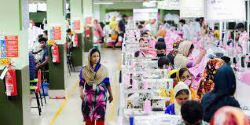
\includegraphics{tex.jpg}}
\caption{Womens In This Sector.}
\label{fig}
\end{figure}

Figure Labels: The readymade garments sector has paved the path for the development of that section of the society, which has been limited to the private sphere, i.e., women. Bangladesh being a developing state has not been able to provide the amenities required for the progress of women like, education, jobs, etc. But with the advent of the RMG factories, many women were able to utilize their proficiency and aptitude for the betterment of the family, society and country. Women, from lower to lower middle class in the urban and rural regions, are being employed in huge numbers in these garment factories (Figure-I). This has served to be the basic means of earning for these women.

\begin{figure}[htbp]
\centerline{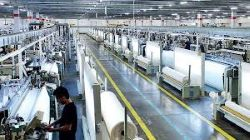
\includegraphics{tex 1.jpg}}
\caption{Auto Machines.}
\label{fig}
\end{figure}

Figure Labels: Various types of machines used in the apparel industry from Warehouse to finishing. In this article, you will get a list of machinery and their functions in the apparel industry.  Hopefully, this list of all the machinery of the apparel industry with their uses will help you to understand the different machine functions. This list contains all types of Garments machinery.For the pattern making of the sample products, you may be interested in software. For this, you can purchase CAD (computer-aided design). There are other components of the CAD systems – pattern grading, Marker planning, Nesting, Pattern digitization. For printing the marker paper, you need a plotter machine. With the help of CAD software, you can estimate fabric requirements accurately and improve the garment fit.

\section*{Acknowledgement}

First and foremost, we would like to thank Almighty Allah for enabling us to initiate the research Paper, to put our best efforts and successfully conclude it. Secondly, we submit our heartiest gratitude to our respected Supervisor Md. Al-Hasan, Lecturer, Department of Computer Science and Engineering in Bangladesh Army University of Science and Technology for his contribution, guidance and support in conducting the research and preparation of the report. Starting from instilling in us the deadliest of fears to the kindest words of inspiration has permitted us to effectively complete the paper. We are truly grateful to him. We revere the patronage and moral support extended with love, by our parents as well as our friends. They helped us with their direct or indirect suggestions which aided in achieving our goal. We would also like to acknowledge the assistance we received from numerous resources over the Internet especially from fellow researchers’ work.
The thesis has also benefited from the comments and suggestions made by Prof. Hasan Muhammad Kafi ,Assistant Professor , Computer Science and Engineering, Bangladesh Army University of Science and Technology. We want to take this opportunity to thanks him.


\begin{thebibliography}{00}
\bibitem{b1} Wikipedia, the free encyclopedia, ``Textile Industry in Bangladesh'' 
\bibitem{b2} https://www.textiletoday.com.bd/textile-industries-in-bangladesh-a-rising-environmental-degradation/#:~:text=Currently%2C%20the%20textile%20industry%20in%20Bangladesh%20accounts%20for,and%20apparel%2C%20according%20to%20the%20latest%20figures%20available.
\bibitem{b3} https://www.dragonsourcing.com/current-scenario-of-the-textile-industry-in-bangladesh/
\bibitem{b4} https://textilelearner.net/future-of-textile-industry-in-bangladesh/
\bibitem{b5}https://www.fibre2fashion.com/industry-article/6944/current-scenario-of-the-textile-industry-in-bangladesh

\end{thebibliography}
\vspace{12pt}
%\color{red}


\end{document}
